\chapter{Geometry}

\section{Geometric primitives}
	% \kactlimport{Point.h}
	% \kactlimport{lineDistance.h}
	% \kactlimport{SegmentDistance.h}
	% \columnbreak
	% \kactlimport{SegmentIntersection.h}
	% \kactlimport{lineIntersection.h}
	% \kactlimport{sideOf.h}
	% \kactlimport{OnSegment.h}
	% \kactlimport{linearTransformation.h}
	% \kactlimport{Angle.h}
	
	\kactlimport{Angle.java}
	\kactlimport{CanonicalAngle.h}
	\kactlimport{PositiveAngle.h}
	\kactlimport{Point.java}
	\kactlimport{Segment.java}
	\kactlimport{Polygon.java}
	\kactlimport{Circle.java}
	\kactlimport{Line.java}
	\kactlimport{Ray.java}
	\kactlimport{Vector.java}
	\centerline{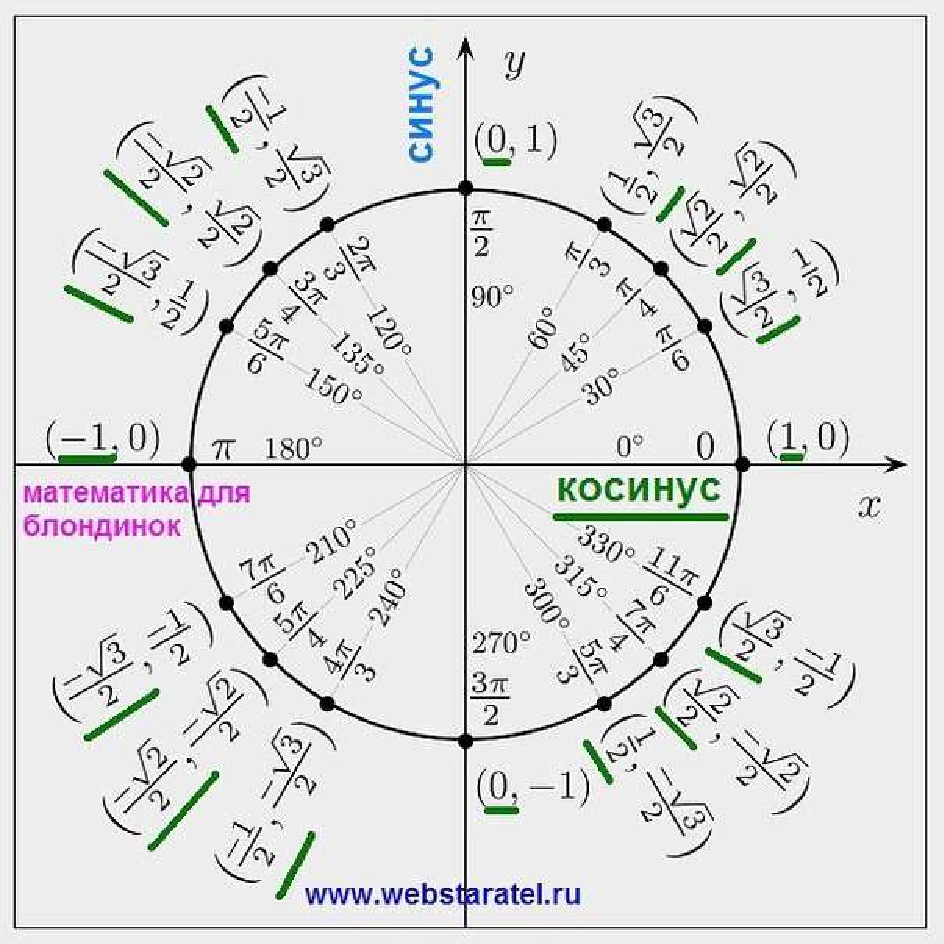
\includegraphics[width=75mm]{content/geometry/TrigonometricAngles}}
	\centerline{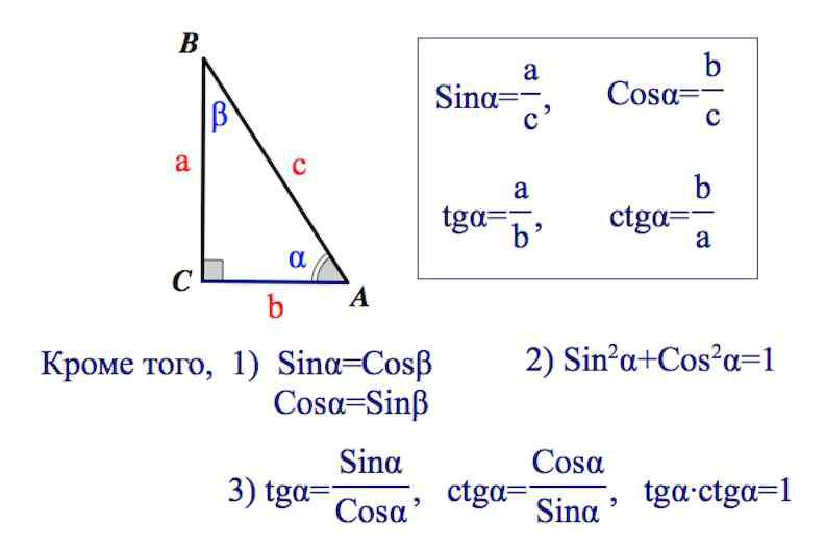
\includegraphics[width=75mm]{content/geometry/TrigonometricTriangles}}

\section{Circles}
	% \kactlimport{CircleIntersection.h}
	% \kactlimport{CircleTangents.h}
	\kactlimport{circumcircle.h}
	\kactlimport{MinimumEnclosingCircle.h}

\section{Polygons}
	% \kactlimport{InsidePolygon.h}
	% \kactlimport{PolygonArea.h}
	% \kactlimport{PolygonCenter.h}
	\kactlimport{PolygonCut.h}
	% \kactlimport{ConvexHull.h}
	% \kactlimport{HullDiameter.h}
	\kactlimport{PointInsideHull.h}
	\kactlimport{LineHullIntersection.h}

\section{Misc. Point Set Problems}
	\kactlimport{ClosestPair.h}
	\kactlimport{kdTree.h}
	% \kactlimport{DelaunayTriangulation.h}
	\kactlimport{FastDelaunay.h}

\section{3D}
	\kactlimport{PolyhedronVolume.h}
	\kactlimport{Point3D.h}
	\kactlimport{3dHull.h}
	\kactlimport{sphericalDistance.h}
